\documentclass{beamer}
\usepackage{amsfonts,amsmath,oldgerm}
\usetheme{sintef}
\usepackage{xeCJK}
\usepackage{tikz}

\newcommand{\testcolor}[1]{\colorbox{#1}{\textcolor{#1}{test}}~\texttt{#1}}

\usefonttheme[onlymath]{serif}

\titlebackground*{assets/Background}

\newcommand{\hrefcol}[2]{\textcolor{cyan}{\href{#1}{#2}}}

\title{Project 3: Search and Convergence}

\subtitle{Theme: Binary Search}
\author{By Elias Alaoui, Enzo Baurianne and Hassan Goulamaly}
\date{Wednesday 14th of January 2026}

\begin{document}
\maketitle


\section{Introduction}
\footlinecolor{sintefyellow}

\begin{frame}{Context \& Objectives}
    \begin{itemize}
        \setlength\itemsep{1em} % Espacement pour plus de lisibilité
        
        \item \textbf{The Problem of Scale:} 
        In the age of Big Data, searching for information is fundamental. A simple linear scan ($O(N)$) becomes unusable as data grows (e.g., searching among 7 billion humans). \pause

        \item \textbf{The Solution:} 
        Binary Search (or Dichotomy) leverages sorted data to eliminate half the search space at every step, offering logarithmic efficiency ($O(\log N)$). \pause

        \item \textbf{Project Goals:}
        \begin{itemize}
            \item \textbf{Implement} the algorithm iteratively in Python.
            \item \textbf{Visualize} the convergence using automated TikZ generation.
            \item \textbf{Prove} correctness and complexity mathematically.
            \item \textbf{Measure} the real-world performance speedup.
        \end{itemize}
    \end{itemize}
\end{frame}

\section{Algorithmic approach}
%-------------------------------------------------------

\begin{frame}{The Principle of Dichotomy}
Searching with Dichotomy is similar to looking for a word in a dictionary:
\begin{itemize}
\item Start in the middle
\item Compare the letter you get with the one you want
\item Open the right or left half in the middle
\item Repeat until you find your word

\end{itemize}
\end{frame}
%--------------------------------------------------------

\begin{frame}[fragile, shrink]{Binary Search Implementation}
    \begin{block}{Python Code}
\begin{verbatim}
def binary_search(sorted_list, target):
    low = 0
    high = len(sorted_list) - 1
    steps = 0

    while low <= high:
        mid = (low + high) // 2
        mid_value = sorted_list[mid]
        steps += 1

        if mid_value == target:
            return mid, steps  # Return index and step count
        elif target > mid_value:
            low = mid + 1
        else:
            high = mid - 1

    return -1, steps
\end{verbatim}
    \end{block}
\end{frame}
%--------------------------------------------------------

\begin{frame}{The Interval Visualizer}
    \centering
    \vfill
    % Code automatically generated by Python
    \begin{tikzpicture}[scale=0.8, transform shape]
      % Nodes style
      \tikzstyle{mybox} = [draw, minimum size=0.8cm, align=center]
      \only<1>{
        \node[mybox, fill=white] at (0, 0) {14};
        \node[font=\tiny, text=gray] at (0, -0.6) {0};
        \node[mybox, fill=white] at (1, 0) {25};
        \node[font=\tiny, text=gray] at (1, -0.6) {1};
        \node[mybox, fill=white] at (2, 0) {31};
        \node[font=\tiny, text=gray] at (2, -0.6) {2};
        \node[mybox, fill=white] at (3, 0) {46};
        \node[font=\tiny, text=gray] at (3, -0.6) {3};
        \node[mybox, fill=orange!50] at (4, 0) {52};
        \node[font=\tiny, text=gray] at (4, -0.6) {4};
        \node[mybox, fill=white] at (5, 0) {63};
        \node[font=\tiny, text=gray] at (5, -0.6) {5};
        \node[mybox, fill=white] at (6, 0) {71};
        \node[font=\tiny, text=gray] at (6, -0.6) {6};
        \node[mybox, fill=white] at (7, 0) {84};
        \node[font=\tiny, text=gray] at (7, -0.6) {7};
        \node[mybox, fill=white] at (8, 0) {96};
        \node[font=\tiny, text=gray] at (8, -0.6) {8};
        \node[mybox, fill=white] at (9, 0) {99};
        \node[font=\tiny, text=gray] at (9, -0.6) {9};
        \node[anchor=north] at (5.0, -1.5) {Step 1: low=0, high=9, mid=4 (Value: 52)};
      }
      \only<2>{
        \node[mybox, fill=gray!30, text=gray] at (0, 0) {14};
        \node[font=\tiny, text=gray] at (0, -0.6) {0};
        \node[mybox, fill=gray!30, text=gray] at (1, 0) {25};
        \node[font=\tiny, text=gray] at (1, -0.6) {1};
        \node[mybox, fill=gray!30, text=gray] at (2, 0) {31};
        \node[font=\tiny, text=gray] at (2, -0.6) {2};
        \node[mybox, fill=gray!30, text=gray] at (3, 0) {46};
        \node[font=\tiny, text=gray] at (3, -0.6) {3};
        \node[mybox, fill=gray!30, text=gray] at (4, 0) {52};
        \node[font=\tiny, text=gray] at (4, -0.6) {4};
        \node[mybox, fill=white] at (5, 0) {63};
        \node[font=\tiny, text=gray] at (5, -0.6) {5};
        \node[mybox, fill=white] at (6, 0) {71};
        \node[font=\tiny, text=gray] at (6, -0.6) {6};
        \node[mybox, fill=orange!50] at (7, 0) {84};
        \node[font=\tiny, text=gray] at (7, -0.6) {7};
        \node[mybox, fill=white] at (8, 0) {96};
        \node[font=\tiny, text=gray] at (8, -0.6) {8};
        \node[mybox, fill=white] at (9, 0) {99};
        \node[font=\tiny, text=gray] at (9, -0.6) {9};
        \node[anchor=north] at (5.0, -1.5) {Step 2: low=5, high=9, mid=7 (Value: 84)};
      }
      \only<3>{
        \node[mybox, fill=gray!30, text=gray] at (0, 0) {14};
        \node[font=\tiny, text=gray] at (0, -0.6) {0};
        \node[mybox, fill=gray!30, text=gray] at (1, 0) {25};
        \node[font=\tiny, text=gray] at (1, -0.6) {1};
        \node[mybox, fill=gray!30, text=gray] at (2, 0) {31};
        \node[font=\tiny, text=gray] at (2, -0.6) {2};
        \node[mybox, fill=gray!30, text=gray] at (3, 0) {46};
        \node[font=\tiny, text=gray] at (3, -0.6) {3};
        \node[mybox, fill=gray!30, text=gray] at (4, 0) {52};
        \node[font=\tiny, text=gray] at (4, -0.6) {4};
        \node[mybox, fill=orange!50] at (5, 0) {63};
        \node[font=\tiny, text=gray] at (5, -0.6) {5};
        \node[mybox, fill=white] at (6, 0) {71};
        \node[font=\tiny, text=gray] at (6, -0.6) {6};
        \node[mybox, fill=gray!30, text=gray] at (7, 0) {84};
        \node[font=\tiny, text=gray] at (7, -0.6) {7};
        \node[mybox, fill=gray!30, text=gray] at (8, 0) {96};
        \node[font=\tiny, text=gray] at (8, -0.6) {8};
        \node[mybox, fill=gray!30, text=gray] at (9, 0) {99};
        \node[font=\tiny, text=gray] at (9, -0.6) {9};
        \node[anchor=north] at (5.0, -1.5) {Step 3: low=5, high=6, mid=5 (Value: 63)};
      }
      \only<4>{
        \node[mybox, fill=gray!30, text=gray] at (0, 0) {14};
        \node[font=\tiny, text=gray] at (0, -0.6) {0};
        \node[mybox, fill=gray!30, text=gray] at (1, 0) {25};
        \node[font=\tiny, text=gray] at (1, -0.6) {1};
        \node[mybox, fill=gray!30, text=gray] at (2, 0) {31};
        \node[font=\tiny, text=gray] at (2, -0.6) {2};
        \node[mybox, fill=gray!30, text=gray] at (3, 0) {46};
        \node[font=\tiny, text=gray] at (3, -0.6) {3};
        \node[mybox, fill=gray!30, text=gray] at (4, 0) {52};
        \node[font=\tiny, text=gray] at (4, -0.6) {4};
        \node[mybox, fill=gray!30, text=gray] at (5, 0) {63};
        \node[font=\tiny, text=gray] at (5, -0.6) {5};
        \node[mybox, fill=orange!50] at (6, 0) {71};
        \node[font=\tiny, text=gray] at (6, -0.6) {6};
        \node[mybox, fill=gray!30, text=gray] at (7, 0) {84};
        \node[font=\tiny, text=gray] at (7, -0.6) {7};
        \node[mybox, fill=gray!30, text=gray] at (8, 0) {96};
        \node[font=\tiny, text=gray] at (8, -0.6) {8};
        \node[mybox, fill=gray!30, text=gray] at (9, 0) {99};
        \node[font=\tiny, text=gray] at (9, -0.6) {9};
        \node[anchor=north] at (5.0, -1.5) {Step 4: low=6, high=6, mid=6 (Value: 71)};
      }
    \end{tikzpicture}

    \vfill
    \begin{itemize}
        \item \textbf{In gray}: The eliminated search areas.
        \item \textbf{In orange}: The central element being compared (\textit{mid}).
    \end{itemize}
\end{frame}
%--------------------------------------------------------

\begin{frame}{Common Error: The "Off-by-One" Error}
    \begin{block}{What is it?}
        A logic error where an iterative algorithm iterates one time too many or too few. In Binary Search, this is the most common source of bugs.
    \end{block} \pause

    \begin{itemize}
        \item \textbf{The Infinite Loop Risk:} 
        \begin{itemize}
            \item Happening if we update bounds incorrectly (e.g., \texttt{low = mid}).
            \item The search space never shrinks to zero.
        \end{itemize} \pause
        
        \item \textbf{The Missing Element:}
        \begin{itemize}
            \item Happening if we use \texttt{while low < high}.
            \item The algorithm terminates before checking the final remaining element.
        \end{itemize} \pause
        
        \item \textbf{The Fix:} Always exclude \texttt{mid} from the new range:
        \begin{itemize}
            \item \texttt{high = mid - 1}
            \item \texttt{low = mid + 1}
        \end{itemize}
    \end{itemize}
\end{frame}
%------------------------------------------------------

\begin{frame}[fragile]{Validation of the algorithm}
    \begin{colorblock}[white]{sintefyellow}{Python Code}
    \tiny
\begin{verbatim}
    def test_binary_search():
        # Test empty list
        assert binary_search([], 5) == -1

        # Test target at the beginning
        assert binary_search([1, 2, 3, 4, 5], 1) == 0

        # Test target at the end
        assert binary_search([1, 2, 3, 4, 5], 5) == 4

        # Test target absent
        assert binary_search([1, 2, 3, 4, 5], 6) == -1

        # Test list with duplicate values
        assert binary_search([1, 2, 2, 2, 3], 2) in [1, 2, 3]  # could return any index of the duplicates

        print("All tests passed.")
\end{verbatim}
    \end{colorblock}    
\end{frame}
%-----------------------------------------------------

\section{Mathematical study}

\begin{frame}[fragile]{Proof of Correctness (Loop Invariant)}
\begin{block}{Loop Invariant $\mathcal{P}$}
        "If target $x$ exists in $L$, then $\text{index}(x) \in [\text{low}, \text{high}]$."
    \end{block} \pause

    \begin{itemize}
        \item \textbf{Initialization:} At start, $[\text{low}, \text{high}]$ is the full list. If $x \in L$, it is necessarily inside. $\mathcal{P}$ holds. \pause
        \item \textbf{Preservation:}
        \begin{itemize}
            \item If $L[\text{mid}] < x$: Sorted list $\implies x$ cannot be in left half. We set $\text{low} = \text{mid} + 1$.
            \item If $L[\text{mid}] > x$: Sorted list $\implies x$ cannot be in right half. We set $\text{high} = \text{mid} - 1$.
        \end{itemize} \pause
        \item \textbf{Conclusion:} We only discard parts where $x$ \textit{cannot} be. $\mathcal{P}$ is preserved.
    \end{itemize}
\end{frame}
%------------------------------------------------------

\begin{frame}{Termination Proof}
    \begin{block}{Why does it stop?}
        We must prove that the search space size $S = (high - low)$ strictly decreases at each step.
    \end{block} \pause

    \begin{itemize}
        \setlength\itemsep{1em}
        \item At each iteration, we update the bounds:
        \begin{itemize}
            \item Either $low = mid + 1$
            \item Or $high = mid - 1$
        \end{itemize} \pause
        \item In both cases, the element at index $mid$ is excluded from the new interval. \pause
        \item The number of candidates strictly decreases. Since the list is finite, the loop condition $low \le high$ will eventually become false.
    \end{itemize}
    
    \begin{center}
        $\Rightarrow$ \textbf{The algorithm is guaranteed to terminate.}
    \end{center}
\end{frame}

%------------------------------------------------------
\begin{frame}{Complexity Analysis}
    \begin{block}{Recurrence Relation}
        Let $T(n)$ be the number of comparisons for a list of size $n$.
        $$ T(n) \approx T(n/2) + 1 $$
        (1 comparison + problem size divided by 2)
    \end{block} \pause
    \scriptsize
    \begin{itemize}
        \setlength\itemsep{1em}
        \item \small \textbf{General Case (Exact Steps):}
        Since $n$ is not always a power of 2, the number of steps $k$ is the smallest integer such that $2^k \ge n$.
        $$ k = \lfloor \log_2(n) \rfloor + 1 $$
        Where $\lfloor x \rfloor$ is the integer part (floor) of $x$. \pause
        \item \textbf{Worst Case Complexity:}
        $$ O(\log_2 n) $$
    \end{itemize}
\end{frame}
%-----------------------------------------------------------


\begin{frame}{Example: Searching the World Population}
    % Introduction du problème
    Imagine we assign for each human an ID which is a simple counter (1st human born = ID:1). \pause
    
    \vspace{0.3cm}
    
    \begin{itemize}
        \item \textbf{Linear Search:} To find a person, we make at most \textbf{7 billion comparisons}. This is extremely long. \pause
        \item \textbf{Binary Search:} We divide the possibilities by two for each comparison ($\log_2$). The search space shrinks rapidly.
    \end{itemize} \pause

    % Le calcul mathématique dans un bloc pour le mettre en valeur
    \begin{block}{Calculation: How many steps ($k$) for 7 billion?}
        We look for $k$ such that $2^k \ge N$ (where $N \approx 7,000,000,000$).
        
        \small % Réduit légèrement la taille pour que tout tienne bien
        \begin{itemize}
            \item \textbf{Approximation:} $2^{10} \approx 1,000 \Rightarrow 2^{20} \approx 10^6 \Rightarrow 2^{30} \approx 10^9$ (1 billion)
        \end{itemize} 

    \end{block}
\end{frame}

%---------------------------------------------------------

\begin{frame}{Example: Searching the World Population}
 
    \begin{block}{Calculation: How many steps ($k$) for 7 billion?}
        \begin{itemize}
        \item \textbf{Testing higher powers:}
            \begin{itemize}
                \item $2^{31} \approx 2.1$ billion
                \item $2^{32} \approx 4.3$ billion (Not enough for 7 billion)
                \item $2^{33} \approx 8.6$ billion (Enough!)
            \end{itemize}
        \end{itemize}
        
        \vspace{0.2cm}
        Since $7 \times 10^9$ is between $2^{32}$ and $2^{33}$, we have $k \approx 32.7$.
        We round up because we cannot do "0.7" of a comparison.
        \vspace{0.1cm}
        
        \centering \textbf{\large Total comparisons needed: 33}

    \end{block}
\end{frame}

%---------------------------------------------------------

\section{Performance}

\begin{frame}{Experimental Results}
    \centering
    % Increased text size to \small and added more padding between columns
    \small 
    \setlength{\tabcolsep}{8pt} 
    \renewcommand{\arraystretch}{1.4} % More vertical space between rows

    \begin{tabular}{|c|c|c|c|c|c|}
        \hline
        \textbf{N} & \textbf{Lin. Time} & \textbf{Lin. Steps} & \textbf{Bin. Time} & \textbf{Bin. Steps} & \textbf{Speedup} \\ 
        \hline
        $10^4$ & 0.000567 & 5,112 & 0.000004 & 12 & 153x \\ 
        $10^5$ & 0.006523 & 48,181 & 0.000010 & 16 & 639x \\ 
        $10^6$ & 0.057961 & 486,187 & 0.000013 & 19 & 4,501x \\ 
        $10^7$ & 0.891410 & 5,052,077 & 0.000021 & 22 & 42,578x \\ 
        \hline
    \end{tabular}
    
    \vspace{0.5cm}
    % Using \textit directly as caption to avoid floating issues
    \textit{Table: Performance comparison (average of 100 searches)}
\end{frame}
%--------------------------------------------------------------

\begin{frame}[fragile]{Performance Comparison Code}
    \begin{colorblock}[white]{sintefyellow}{Python Code}
    
    \tiny
\begin{verbatim}
def linear_search(sorted_list, target):
    steps = 0
    for index, value in enumerate(sorted_list):
        steps += 1
        if value == target:
            return index, steps
    return -1, steps

def performance_comparison():
    list_sizes = [10 ** 4, 10 ** 5, 10 ** 6, 10 ** 7]
    num_searches = 100

    print("=" * 115)
    print("PERFORMANCE COMPARISON (Average of 100 searches)")
    print("=" * 115)
    print(
        f"{'List Size (N)':<15} {'Lin. Time(s)':<15} {'Lin. Steps':<15}"
        f" {'Bin. Time(s)':<15} {'Bin. Steps':<15} {'Speedup'}")
    print("-" * 115)
\end{verbatim}
    \end{colorblock}
\end{frame}
%------------------------------------------------------

\begin{frame}[fragile, shrink]{Performance Comparison Code}
    \begin{colorblock}[white]{sintefyellow}{Python Code}
    \scriptsize 
\begin{verbatim}
    for size in list_sizes:
        sorted_list = list(range(size))

        total_linear_time = 0
        total_binary_time = 0
        total_linear_steps = 0
        total_binary_steps = 0

        for search_index in range(num_searches):
            target = random.randint(0, size - 1)

            # Time Linear Search
            start_time = timeit.default_timer()
            search_index, steps = linear_search(sorted_list, target)
            total_linear_time += timeit.default_timer() - start_time
            total_linear_steps += steps

            # Time Binary Search
            start_time = timeit.default_timer()
            search_index, steps = binary_search(sorted_list, target)
            total_binary_time += timeit.default_timer() - start_time
            total_binary_steps += steps
\end{verbatim}
    \end{colorblock}
\end{frame}
%------------------------------------------------

\begin{frame}[fragile, shrink]{Performance Comparison Code}
    \begin{colorblock}[white]{sintefyellow}{Python Code}
    \scriptsize 
\begin{verbatim}
        # Calculate Averages
        avg_linear_time = total_linear_time / num_searches
        avg_binary_time = total_binary_time / num_searches
        avg_linear_steps = total_linear_steps / num_searches
        avg_binary_steps = total_binary_steps / num_searches

        # Avoid division by zero for extremely fast operations
        if avg_binary_time > 0:
            speedup = avg_linear_time / avg_binary_time
        else:
            speedup = float('inf')

        # Print Row
        print(
f"{size:<15,d} {avg_linear_time:<15.6f} "
                        f"{avg_linear_steps:<15.0f} {avg_binary_time:<15.6f} "
                        f"{avg_binary_steps:<15.0f} {speedup:,.0f}x")

    print("=" * 115
\end{verbatim}
    \end{colorblock}
\end{frame}
%------------------------------------------------

\definecolor{sorbonneblue}{RGB}{8, 50, 136}
\section{Conclusion}

\begin{frame}{Conclusion}
    \begin{itemize}
        \setlength\itemsep{1.5em} % Plus d'espace car il y a moins de texte
        
        \item \textbf{Theoretical Validation:} 
        Correctness proven via Loop Invariant and $O(\log N)$ complexity confirmed.
        \pause

        \item \textbf{Experimental Results:} 
        Achieved a massive speedup of over \textbf{42,000x} compared to Linear Search.
        \pause

        \item \textbf{Visualization:}
        Automated TikZ clearly illustrates the rapid "Divide and Conquer" convergence.
        \pause

        \item \textbf{Key Takeaway:} 
        Binary Search is not just faster; it is \textbf{essential} for Big Data scalability.
    \end{itemize}
\end{frame}

\end{document}
